\documentclass[paper=letter, fontsize=12pt]{article}
\usepackage{geometry}
\geometry{margin=1in}
\usepackage{graphicx}
\graphicspath{{images/}}
\usepackage{amssymb}
\usepackage{enumitem}
\usepackage{amsmath}
\usepackage{mathrsfs}

%opening
\title{Compsci 571 HW5}
\author{Yilin Gao (yg95)}

\begin{document}

\maketitle
\section{Hoeffding's Inequality}

\begin{enumerate}[label=(\alph*)]
	%1a
	\item 
	For all $t \geq 0$,
	
	$$Pr(\frac{1}{n}\sum_{i=1}^{n}(X_i-\mu_{X_i})\geq t) = Pr(\sum_{i =1}^{n} (X_i - \mu_{X_i}) \geq nt)$$
	
	Because $X_1, \dots, X_n$ are independent random variables, $\sum_{i = 1}^{n} X_i$ is also a random variable, and its mean is $E[\sum_{i = 1}^{n} X_i] = \sum_{i = 1}^{n} E(X_i) = \sum_{i = 1}^{n} \mu_{X_i}$. Denote $X' = \sum_{i = 1}^{n} X_i$, and $\mu_{X'} = E[X']$.
	
	So the above probability is:
	
	$$ = Pr(X' - \mu_{X'} \geq nt)$$

	According to Chernoff Bounds:
	
	$$\leq \min_{\lambda \geq 0} M_{X' - \mu_{X'}} (\lambda) e^{-\lambda nt} = \min_{\lambda \geq 0} E[e^{\lambda (X' - \mu_{X'})}] e^{-\lambda nt} = \min_{\lambda \geq 0} E[e^{\lambda \sum_{i = 1}^{n}(X_i - \mu_{X_i})}] e^{-\lambda nt}$$	
	
	$$= \min_{\lambda \geq 0} E[\prod_{i = 1}^{n} e^{\lambda (X_i - \mu_{X_i})}] e^{-\lambda nt} = \min_{\lambda \geq 0} (\prod_{i = 1}^{n} E[e^{\lambda (X_i - \mu_{X_i})}]) e^{-\lambda nt}$$
	
	Apply Hoeffding's Lemma to each $X_i, i = 1, \dots, n$:
	
	$$\leq \min_{\lambda \geq 0} ( \prod_{i = 1}^{n} \exp(\frac{\lambda^2 (b-a)^2}{8})) \exp(-\lambda nt) = \min_{\lambda \geq 0} \exp(\sum_{i = 1}^{n} \frac{\lambda^2(b-a)^2}{8}) \exp(-\lambda nt)$$
	
	$$= \min_{\lambda \geq 0} \exp(\frac{n \lambda^2 (b-a)^2}{8} - \lambda nt)$$
	
	Because the exponential function is increasing on its argument, so its minimal value occurs at its minimal argument value.
	
	For $\frac{n \lambda^2 (b-a)^2}{8} - \lambda nt$, when $\lambda^* = \frac{4t}{(b-a)^2} (\geq 0)$, its minimal value is $- \frac{2nt^2}{(b-a)^2}$.
	
	So we got $\min_{\lambda \geq 0} \exp(\frac{n \lambda^2 (b-a)^2}{8} - \lambda nt) = \exp(- \frac{2nt^2}{(b-a)^2})$. $\ \ \square$
	
	%1b
	\item
\end{enumerate}

\section{VC Dimension}

\begin{enumerate}[label=(\alph*)]
	%2a
	\item 
	The VC dimension of $\mathcal{H}_1$ is $p$, because its feature space is $p$-dimensional, and all separating hyperplanes are linear in the feature space and goes though the origin point.
	
	The VC dimension of $\mathcal{H}_2$ is $\frac{(p+2)(p+1)}{2}$, because its feature space is $\frac{(p+2)(p+1)}{2}$-dimensional, and all separating hyperplanes are linear in the feature space and goes though the origin point.
	
	%2b
	\item The approximation and estimation errors for $\mathcal{H}_1$, $\mathcal{H}_2$ and $\hat{f}_1$, $\hat{f}_2$ are depicted as following:
	
	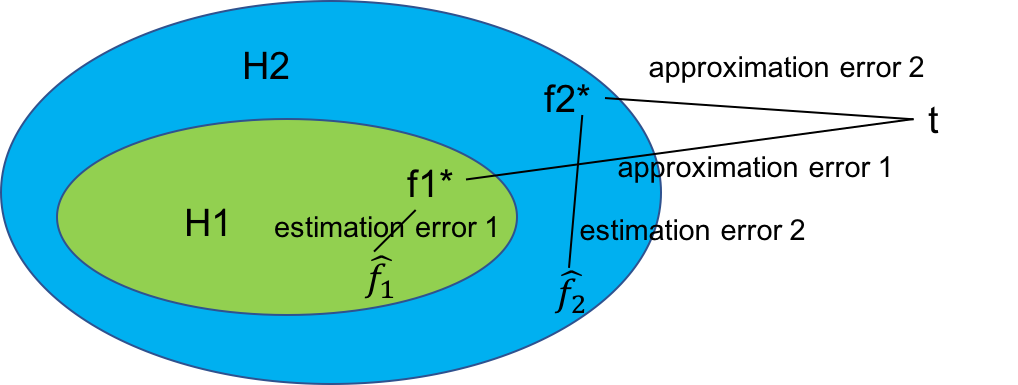
\includegraphics[scale=0.6]{q2b.png}
	
	In the picture, $t$ stands for the global optimal function based on true risk, $f_1^*$ and $f_2^*$ stand for the optimal functions based on true risk in function classes $\mathcal{H}_1$ and $\mathcal{H}_2$ respectively, and $\hat{f}_1$ and $\hat{f}_2$ are optimal functions based on empirical risk in function classes $\mathcal{H}_1$ and $\mathcal{H}_2$ respectively.
	
	As $n$ increases, the estimation error increases because with more data we are able to estimate the model more accurately, and decrease the discrepancy between true risk and empirical risk, i.e., the estimation error. And the approximation error won't be affected significantly because the approximation error is dependent on the function class $\mathcal{H}$, but not the data.
	
	%2c
	\item One function class $\mathcal{F}$ such that its VC dimension is not equal to its number of parameters is the set of functions generated by the K-nearest nerighbors algorithm with $K=1$. It only has 1 parameter $K$, while its VC dimension is infinity (because with $K=1$ it classifies every data point into the class same as its true class, thus being able to shatter any number of data points).
\end{enumerate}

\section{Ridge Regression}

\begin{enumerate}[label=(\alph*)]
	%3a
	\item Denote $f(\beta) = \sum_{i = 1}^{n} \Vert \boldsymbol{y} - \boldsymbol{X} \beta \Vert_2^2 + \lambda \Vert \beta \Vert_2^2$
	
	$$\frac{d f(\beta)}{d \beta_j} = -2 \boldsymbol{x}_{\cdot j}^T (\boldsymbol{y} - \boldsymbol{X} \beta ) + 2 \lambda \beta_j$$
	
	$$\frac{\nabla f(\beta)}{\nabla \beta} = -2 \boldsymbol{X}^T (\boldsymbol{y} - \boldsymbol{X} \beta) + 2 \lambda \beta = 0$$
	
	We get:
	
	$$\hat{\beta}^{ridge} = (\boldsymbol{X}^T \boldsymbol{X} + \lambda \boldsymbol{I})^{-1} \boldsymbol{X}^T \boldsymbol{y}$$ in which $\boldsymbol{I}$ is a $p \times p$ diagonal matrix with 1's as its diagonal values.
	
	%3b
	\item The plot of average ridge MSE with respect to $\lambda \in [0, 10]$ for both $\beta_1$ and $\beta_2$ is:
	
	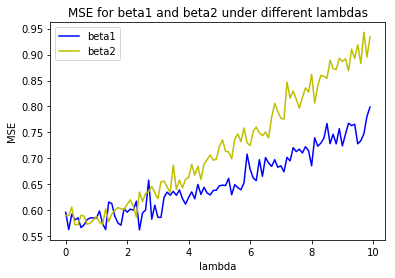
\includegraphics[scale=0.6]{q3b.png}
	
	From the plot we can see:
	
	\begin{enumerate}[label=(\arabic*)]
		\item As $\lambda$ increases, the MSEs of both $\beta_1$ and $\beta_2$ increase. This is because $\lambda$ will force regression estimated coefficients $\hat{\beta}$ to be not too large to avoid overfitting, thus leading to imprecise prediction. When $\lambda$ is larger, the bias in estimated coefficient $\hat{\beta}$ will be larger, so will the MSE be.
		
		\item For the same $\lambda$ value, the MSE of $\beta_2$ is larger than that of $\beta_1$ in general. This is because values in $\beta_2^*$ are larger than those in $\beta_1^*$. So their unbiased estimated values will also be larger. With regularization, their estimated values will be shrunk more, so the training MSE will be larger for $\beta_2$.
	\end{enumerate}
	
	%3c
	\item 
	From the problem setting, we can know that $\mathbf{U}_{p}^{T} \mathbf{U}_{p} = \mathbf{I}_{p}$, $\mathbf{V}^T \mathbf{V} = \mathbf{I}_{p}$, $\mathbf{L} = \mathbf{L}^{T}$. And because $\mathbf{X}^{T} \mathbf{X} = corr(\mathbf{X})$, $\mathbf{U}^{T}_{p}$ is orthogonal to $\mathbf{1}_{p}$, i.e., $\mathbf{U}^{T}_{p} \mathbf{1}_{p} = \mathbf{1}^{T}_{p} \mathbf{U}_{p} = \mathbf{0}_p$.
	
	\begin{eqnarray*}
	\mathbf{U}^T \mathbf{Y} = 
		\begin{bmatrix}
			\mathbf{1}^T_{n} \\
			\mathbf{U}^T_p \\
			\mathbf{U}^{T}_{n-p-1}\\
 		\end{bmatrix} \mathbf{1}_n \alpha
 		+ 
 		\begin{bmatrix}
 		\mathbf{1}^T_{n} \\
 		\mathbf{U}^T_p \\
 		\mathbf{U}^{T}_{n-p-1}\\
 		\end{bmatrix} \mathbf{U}_{p} \mathbf{L} \mathbf{V}^T \beta
 		+ \mathbf{U}^T \epsilon
	\end{eqnarray*}

	\begin{eqnarray*}
	=  \begin{bmatrix}
			n\alpha + \mathbf{1}^T_{n} \mathbf{U}_{p} \mathbf{L} \mathbf{V}^T \beta \\
			\mathbf{U}^T_p \mathbf{1}_n \alpha + \mathbf{U}^T_p \mathbf{U}_{p} \mathbf{L} \mathbf{V}^T \beta \\
			\mathbf{U}^{T}_{n-p-1} \mathbf{1}_n \alpha + \mathbf{U}^{T}_{n-p-1} \mathbf{U}_{p} \mathbf{L} \mathbf{V}^T \beta
		\end{bmatrix} + \mathbf{U}^T \epsilon
	\end{eqnarray*}
	
	\begin{eqnarray*}
	= \begin{bmatrix}
			n\alpha \\
			\mathbf{L} \mathbf{V}^T \beta \\
			\mathbf{U}^{T}_{n-p-1} \mathbf{1}_n \alpha + \mathbf{U}^{T}_{n-p-1} \mathbf{U}_{p} \mathbf{L} \mathbf{V}^T \beta
		\end{bmatrix} + \mathbf{U}^T \epsilon
	\end{eqnarray*}

	At the same time, we have the same equation represented by $\gamma$:
	
	\begin{eqnarray*}
	\mathbf{Y}^* = \mathbf{U}^{T} \mathbf{Y} = 
		\begin{bmatrix}
			n\alpha \\
			\mathbf{L} \gamma \\
			\mathbf{0}_{n-p-1}
		\end{bmatrix} + \mathbf{U}^T \epsilon
	\end{eqnarray*}

	So we have $\mathbf{L} \mathbf{V}^T \beta = \mathbf{L} \gamma$, or $\gamma = \mathbf{V}^{T} \beta$.
	
	From the original function $\mathbf{Y} = \mathbf{1} \alpha + \mathbf{U}_{p} \mathbf{L} \mathbf{V}^{T} \beta + \epsilon$, we get the objective function of ridge regression:
	
	\begin{equation*}
	f(\alpha, \beta) = \Vert \mathbf{Y} - \mathbf{1} \alpha - \mathbf{X} \beta \Vert_2^2 + \lambda [\alpha^2 + \Vert \beta \Vert_2^2]
	\end{equation*}
	
	\begin{equation*}
	\frac{\partial f}{\partial \alpha} = -2 \sum_{i = 1}^{n} (y_i - \alpha - \mathbf{x}_i \beta) + 2 \lambda \alpha = 2(n + \lambda) \alpha -2 \mathbf{1}^{T}_{n} (\mathbf{Y} - \mathbf{X} \beta)  = 0
	\end{equation*}
	
	\begin{equation*}
	\frac{\nabla f}{\nabla \beta} = -2 \mathbf{X}^{T} (\mathbf{Y} - \mathbf{1} \alpha - \mathbf{X} \beta) + 2 \lambda \beta = 0
	\end{equation*}
	
	From the 2 equations, we get $\hat{\beta}^{ridge} = [\mathbf{X}^{T} (\mathbf{I}_n - \frac{1}{n + \lambda} \mathbf{1}_n \mathbf{1}_n^{T}) \mathbf{X} + \lambda \mathbf{I}_p]^{-1} [\mathbf{X}^{T} (\mathbf{I}_{n} - \frac{1}{n + \lambda} \mathbf{1}_n \mathbf{1}_n^{T}) \mathbf{Y}]$.
	
	Since we have $\mathbf{X} = \mathbf{U}_p \mathbf{L} \mathbf{V}^{T}$, $\mathbf{X}^{T} \mathbf{X} = \mathbf{V} \mathbf{L}^2 \mathbf{V}^{T}$, and $\mathbf{X}^{T} \mathbf{1}_{n} = \mathbf{V} \mathbf{L} \mathbf{U}^{T}_{p} \mathbf{1}_n = \mathbf{0}_{p}$.
	
	So $\hat{\beta}^{ridge} = [\mathbf{X}^{T} \mathbf{X} + \lambda \mathbf{I}_p]^{-1} [\mathbf{X}^{T} \mathbf{Y}] = \mathbf{V} (\mathbf{L}^2 + \lambda \mathbf{I}_{p})^{-1} \mathbf{L} \mathbf{U}^{T}_{p} \mathbf{Y}$. 
	
	And $\hat{\gamma}^{ridge} = \mathbf{V}^{T} \hat{\beta}^{ridge} = (\mathbf{L}^2 + \lambda \mathbf{I}_{p})^{-1} \mathbf{L} \mathbf{U}^{T}_{p} \mathbf{Y}$.
\end{enumerate}
\end{document}
